%TEX root = ../dissertation.tex

\chapter{Related Work}
\label{chapter:related-work}

In this section, we will cover the research work and industry references that
can be considered relevant to our initial objective. The following section
\ref{distributed-publish-subscribe-paradigm} will lay the ground to define how
pub-sub systems are structured. In section \ref{relevant-pub-sub-systems} we
will cover a set of systems defined as relevant. Finally, section
\ref{web-technologies} will address some of the web technologies of interest in
this area.

\section{Distributed Publish-Subscribe
Paradigm}\label{distributed-publish-subscribe-paradigm}

In this section we will cover the basis of the pub-sub paradigm, defining a
taxonomy we will later use to classify relevant systems. We will start by
covering the \emph{Subscription Model}, followed by the \emph{Network
Architecture} and \emph{Overlay Structure}. Finally, we
address the \emph{Subscription Management and Event Dissemination}.

\subsection{Subscription Model}\label{subscription-model}

When considering pub-sub systems, there is a set of different options that will
lay ground for the behaviour of the whole system. We call these options, design
dimensions. Specifically, in our case, one of the biggest decisions when
designing a pub-sub system is what kind of subscription model to use.The
subscription model determines how subscribers will define which events they are
interested in. There are three major approaches covered by relevant literature
\cite{Kermarrec2013} \cite{Eugster2003} and that implementations usually
follow:

\begin{itemize}
  \item
    Topic based subscriptions
  \item
    Content based subscriptions
  \item
    Type based subscriptions
\end{itemize}

\textbf{Topic based subscription model} employs, as the name states, the
notion of topics or subjects to allow participants to subscribe to
relevant content. These topics are identified by keywords and can be
naturally viewed as a group or a channel to which participants can send
messages (publish) and receive messages (subscribe). This approach was
one of the earliest models in the pub-sub paradigm, with references
such as TIBCO~\footnote{https://www.tibco.com/}, mainly due to its similarity with the group
communication systems already in place at the time. Some examples of the
topic based approach allow building a topic hierarchy. A specific one is
using a UNIX path like approach, which allows a topic hierarchy
just like paths in a file system. Consider as an example:

\begin{verbatim}
/fruits
/fruits/citrus
/fruits/citrus/orange
\end{verbatim}

The list above is an example of 3 topics, that act as 3 different tiers
on a hierarchy. This allows for specialisation and the possibility to
extend the subscription structure already in place. There are numerous
solutions that cover the topic based subscription scenario. Specifically,
in the distributed/decentralised area, we have solutions like Scribe \cite{Castro2002},
Bayeux \cite{Zhuang2001}, Tera \cite{Baldoni2007} and Poldercast \cite{Setty2012}.
\bigskip

\textbf{The content based subscription model} brought a different
approach that sought to use the content of the event message itself as a
way for subscribers to specify the messages they were interested in \cite{Banavar1999}.
Essentially, subscribers could define fields, or conditions on those same fields that would make an event
match a subscription or not. Consider the following example of a simple
message and subscription, represented using JSON~\footnote{https://www.json.org/}.
\bigskip

\textbf{Message}

\begin{verbatim}
{
  exchange: "Euronext Lisboa",
  company: "CTT",
  order: "buy",
  number: "100",
  price: "5.55",
}
\end{verbatim}

\textbf{Subscription}

\begin{verbatim}
{
  exchange: "Euronext Lisboa",
  order: "buy",
  number: ">50",
  price: "<10",
}
\end{verbatim}

The example above translates into a subscription to a stock exchange
pub-sub system, where the client would receive all the event messages
for \emph{buy orders} of more than 50 stock actions for a maximum price of
10\euro. The notion of subscription is much more complex in this
model but allows for a much more powerful, expressive and accurate
message filtering. Usually, in order to implement this, systems rely on
the definition of schemas as a way to create subscriptions. Some
examples of solutions that follow a content based subscription model are
Gryphon \cite{Strom1998}, Jedi \cite{Cugola2001}, Siena \cite{Carzaniga2003},
Meghdoot \cite{Gupta2004}, Mercury \cite{Bharambe2002} and Sub-2-sub \cite{Voulgaris2005}.
\bigskip

Also worth referencing is the \textbf{type based subscription model}.
\cite{Eugster2000}. The type based model seeks to use the type
scheme of a programming language without introducing a topic hierarchy.
Instead, it focuses on the idea that, in practice, messages part of the
same topic usually are of the same type and notify the same kind of
event. As such we can rely on a straightforward type-safe interpretation
of messages belonging to the same topic, since most topic based systems
only offer, at most, weakly typed interfaces. This, of course, comes
quite handy when working with strongly typed languages such as Java and
C++. One other aspect also worth mentioning is that, similar to topic
based systems, the type based system also offers a notion of hierarchy
through sub-typing. In this area, Hermes \cite{Pietzuch2002} is a
reference system implemented on top of a distributed network.

While looking back at these different models it is crucial to understand
how they are tied to the expressiveness of the system as a whole.
Choosing a topic based subscription model will allow for an easier
implementation when it comes to message filtering at each node, but it
will clearly affect the capabilities of the system. On the other end, a
content based subscription model allows for a lot more expressiveness in
subscription definition, but it makes it a lot harder to implement a
scalable way of filtering messages. It is also important to note that
these three categories are not strict distinct models, but somewhat
fluid and subject to hybridisation, as is quite possible to have
solutions in between, such as content based filtering through the use of
special topics, or content based filtering only for pre-set fields. As
such, not all approaches are easy to categorise and, for some specific
scenarios and systems, the line is quite thin between the multiple
subscription models.

It is also interesting to look at the application space and notice that
not all applications have the same expressiveness requirements. This
makes the existence of multiple subscription models not only justifiable
but required. Consider the example that was given above for a stock exchange
system: this kind of applications have a need for a complex set of
subscription patterns, quite different from the ones you would probably
have for a chat or social media application, which would rely heavily on
the notion of topics and groups.

\subsection{Network Architecture}\label{network-architecture}

Independently of the subscription model used, the system approach to the
network architecture is crucial as it will, not only set the way clients
interact with it, but will also determine a lot of the properties that
the solution will benefit from (such as scalability, reliability, etc.). Networks
can generally be categorised as centralised or decentralised.

\begin{figure}[hb!]
  \centering
  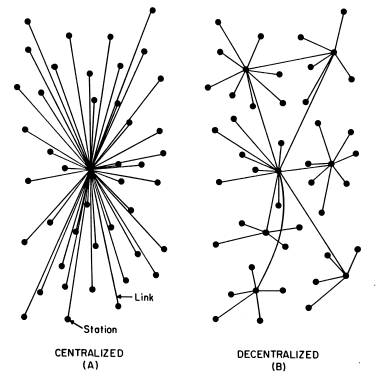
\includegraphics[max height=4cm,max width=0.95\textwidth]{img/network-archs.png}
  \caption{Example of a Centralised and a Decentralised network, extracted from \cite{Baran1964}}
  \label{fig:network-archs}
\end{figure}

Note that the goal of a pub-sub system is to enable the exchange of
events in an asynchronous manner, with the decoupling of producers from
consumers as previously discussed. This can be easily achieved using an
entity which is responsible for receiving the messages from the
producers, storing them and distributing them across all the consumers. This is
what we refer to as a \textbf{centralised architecture}, motivated by the need of
this central entity. This is the approach adopted by a lot of the
message queue systems like Apache Active MQ, RabbitMQ and Redis. The
usual focus for applications relying on this kind of systems is on
reliability and data consistency but with a low data throughput. Typically expected
to operate in a more stable environment, such as datacenters. Figure \ref{fig:centralised-topology}
is an example to illustrate how would a centralised pub-sub system work.

\begin{figure}[hb!]
  \centering
  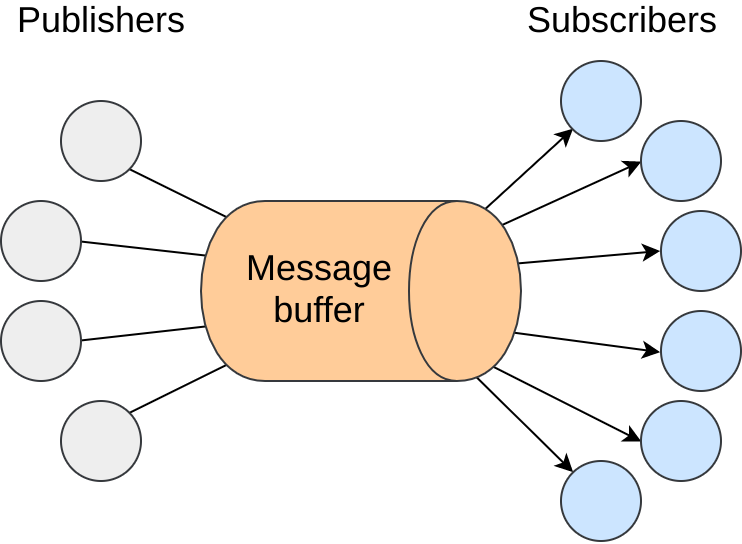
\includegraphics[max height=4cm,max width=0.95\textwidth]{img/centralised-topology.png}
  \caption{Example of a centralised message broker}
  \label{fig:centralised-topology}
\end{figure}

Being the broad term that it is, centralised encompasses a lot of different solutions.
One can have centralised solutions that employ a distribution of load through
different nodes in order to improve the overall scalability of the system. In the pub-sub field, these networks
of servers are commonly referred to as brokers. There are multiple pub-sub systems
that follow this approach. More precisely Gryphon \cite{Strom1998}, Siena \cite{Carzaniga2003}
and Jedi \cite{Cugola2001}. But, even between them, there are some clear differences
on how these broker networks organise. In both Gryphon and Jedi, these nodes organise in
a hierarchical fashion, or define what we call a \textbf{broker hierarchy}. As for Siena,
the nodes resort to not following a specific structure, making it effectively a \textbf{broker mesh}.

The asynchronous nature of the pub-sub paradigm also allows for a
different approach to message forwarding, with both producers and
consumers being responsible for storing and forwarding messages, without
the need of an intermediary entity. This approach is referred to as a
\textbf{decentralised architecture} as there is no central entity that could easily
become a bottleneck for the whole system. Additionally, when the network is
\textbf{fully decentralised} it is commonly referred to as peer to peer (P2P) architecture,
for it relies solely on the communication between peers in the same network.
An example of a pub-sub system following this approach is Scribe \cite{Castro2002}.
This kind of systems have a great focus on scalability and, consequently, on efficient message delivery.

\subsection{Overlay structure}\label{overlay-structure}

Working with a P2P architecture has its own set of challenges. When we
rely on the communication between peers we need a way to create and
maintain links between multiple nodes in a network. Hence the overlay
networks. The idea is to have a structure of logical links and nodes,
independent of the physical network beneath them that actually powers
the communications through. Unlike traditional layer-3 networks, the
structure of these overlays is not dictated by the fairly statical
physical topology (presence and connectivity of hosts), but by logical
relationships between peers. This way we have the potential to
manipulate the logical network at the application level, without needing
to change the network backbone that connects the nodes. This approach
was key to deploy P2P applications such as Gnutella~\footnote{https://web.archive.org/web/20000620113133/http://gnutella.wego.com},
Kazaa~\footnote{https://web.archive.org/web/20040701062605/http://www.kazaa.com:80/us/index.htm}
or Skype~\footnote{https://www.skype.com} on top of the existing Internet infrastructure.

\begin{figure}[hb!]
  \centering
  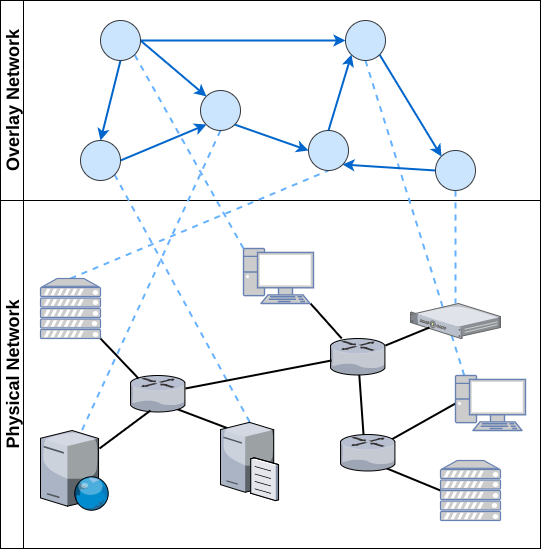
\includegraphics[max height=7cm,max width=0.95\textwidth]{img/overlay-vs-physical.png}
  \caption{A comparison between the physical network and a logical overlay}
  \label{fig:overlay-vs-physical}
\end{figure}

In practical terms, each node maintains a view of its neighbours in the
overlay network, which translates into the communication links between
them. There are different approaches to the way this state is stored and
maintained, with two main categories dominating the P2P ecosystem. At
one end of the spectrum we have the \textbf{unstructured overlay}
networks, where peers form a network with no clear structure or
hierarchy (commonly referred to as a network mesh) with each peer
connected to a subset of other nodes independent of their ID,
localisation, network IP address, etc.
\bigskip

\textbf{Unstructured overlays}: These rely on membership protocols that
try to preserve a couple of key properties, such as the network diameter
and its average degree. A great amount of these membership protocols use
gossip based (also referred to as epidemic) approaches in order to do
this. These approaches exploit properties that arise when information is
disseminated in a random, or close to random, way. These probabilistic
approaches help to keep the overlay connected in the event of network
failures.

One relevant example is Cyclon \cite{Voulgaris2005a}, a membership
protocol that uses a gossip based approach to help maintain a network
which resembles a random graph in
terms of degree distribution, clustering coefficient and path length. In
order to do this, the approach followed by Cyclon is, at each node,
besides keeping a fixed size of neighbours (other nodes in the network),
to also keep information on when for the last time that node was
contacted. Periodically, each node contacts the oldest node of its
neighbours (i.e.~the node which has been the longest time without being
contacted) and shares with it a fixed size partial list of its
neighbours, to which the contacted peer replies back with its own
partial view of its neighbours. Each node updates its neighbours list
with the new info (either by filling empty cache slots or by replacing
entries that were sent in the previous contact). It is also worth noting
that during this exchange, the node that initiated the contact will drop
the contacted node of its neighbour list, as the contacted node will
inversely add the node that established contact to his. This way we end
up with a uniform and organic way to disseminate node information across
the network. This approach is based on a technique named shuffling \cite{Stavrou2002}.

The unstructured overlay has an interesting set of properties, such as
its ability to accommodate a highly dynamic network with a high
resilience to network failures and churn (i.e.~high volumes of changes
in network participants). However, the lack of structure in the network
usually limits the kind of queries for content one can run through. The
delivery of messages in the network will always follow a probabilistic
best effort approach. Finally, unstructured gossip based approaches rely
on a pre-set of conditions that, if not met accordingly, may affect the
whole behaviour of the system \cite{Alvisi2007}. For example, the selection of
neighbours is a key aspect and should assume a random or pseudo-random
fashion. If disturbed by a small set of nodes that could either be
malfunctioning or behaving selfishly, the basic properties of the
network like its resilience could be severely affected.
\bigskip

\textbf{Structured overlays}: On the other end of the spectrum of
overlay networks we have the \textbf{structured overlay}, where peers
are organised according to a specific structure, like a ring, a tree or
a multi-dimensional space. This is usually achieved by imposing
constraints on how the nodes should be organised based on their
identifiers. In order to do this, a common approach is to think of the
ID space as a hash table to where the content should then be
distributed. The distribution of content is then done based the value of
the keys generated for each piece of information, keys with values close
to a node ID will be stored in that node. This is commonly referred to
as a Distributed Hash Table (or DHT for short) since the key space is
distributed across multiple nodes. For example, \textbf{Chord} \cite{Stoica2001},
one of the first examples of a DHT, organises the nodes in a ring like structure
based on their ID (which results from the SHA-1 hash~\footnote{https://tools.ietf.org/html/rfc3174}
of its IP address). The content is then distributed in this key space, using the same hashing function to
produce the content key that was used to produce the node ID.

\begin{figure}[hb!]
  \centering
  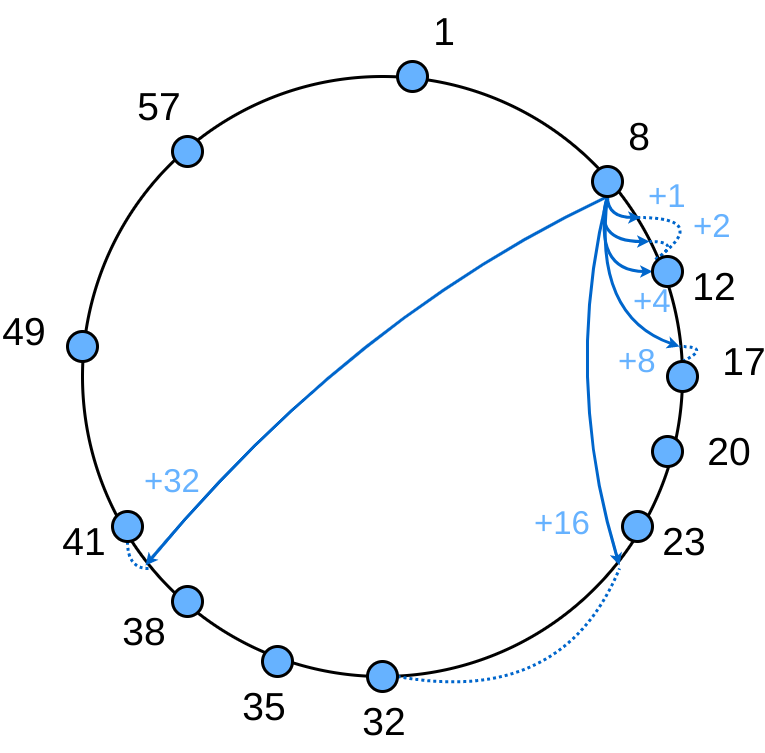
\includegraphics[max height=5cm,max width=0.95\textwidth]{img/chord.png}
  \caption{Example of a simple Chord ring and the finger table of a node}
  \label{fig:chord}
\end{figure}

It is common for Distributed Hash Tables to have a cost of O(log{}N)
in terms of the number of nodes
contacted, on average, to search for a given key (where N is the number
of nodes in the network). Chord base structure per se only gives us
O(N), as such, Chord uses a mechanism to allow for a speedier search. At
each node, an additional routing table is kept with m entries, where m
is the number of bits in the key space. Each $ith$ entry in this table
will be this node's successor (next node in the ring in a clockwise
direction) with an ID, at least, bigger than $2^{i-1}$ (modulo $2^{m}$)
in the key space. For example, for
a node with ID 8, the 4th entry will be the first node in the ring with
an ID larger than 16. This table, also referred to as finger table, will
allow for a logarithmic search as demonstrated in Chord's specification.

Another approach is followed by \textbf{Kademlia DHT} \cite{Maymounkov2002}.
Just as in Chord, nodes have 160 bit identifiers and content is
stored in the nodes whose IDs are close to the content key (160 bit
identifiers too), but the way the routing tables are structured and
maintained is quite different. For starters, Kademlia relies on a XOR
based distance metric between 2 keys, where the distance between 2 keys
is the resulting bitwise XOR operation interpreted as an integer. The
XOR metric gives us an interesting set of properties. It is
unidirectional (just like Chord clockwise direction) ensuring that
lookups for the same key converge along the same path but, unlike Chord,
it is symmetric, as such, the distance between $x$ and $y$ is the same as
the distance between $y$ and $x$. This symmetry allows Kademlia queries to
give valuable insights along every node they go through, helping out in
populating each node's routing table.

Kademlia nodes keep contact information about each other in a list, size
m where m is the number of bits used for the keys in the system, and
where each entry is a list itself of maximum size k (a system wide
parameter) containing all the known nodes of distance between $2^{i}$ and
$2^{i+1}$ of itself. These lists
are appropriately called k-buckets and are kept sorted by time last seen
(least recently seen node at the head). Whenever a node receives a
message, it updates the appropriate k-bucket for the sender's node ID,
inserting it in the respective k-bucket or moving it to the tail of the
list if it is already there. K-buckets aim at implementing a
least-recently seen eviction policy, where live nodes are never removed.
This stems from a careful analysis of Gnutella trace data \cite{Saroiu2002}
where the longer a node has been up, the more likely
it is to remain up for another hour. Whenever a node wants to retrieve
or store content it uses a recursive node lookup procedure in order to
find the k closest nodes to a given key. This lookup can be run with
multiple queries in parallel, because nodes have the flexibility to
forward messages to any of the k nodes in a bucket, aiming for lower
latency.

A completely different method is used in the \textbf{Content Addressable
Network DHT}\cite{Ratnasamy2001a}. In CAN, the key space used to
address the content stored in the DHT is a virtual d-dimensional
Cartesian coordinate space. In order to store and retrieve content, the
generated keys use a uniform hashing function that maps the key into the
d-dimensional space, resulting in a point. The overall space is split
into different areas referred to as zones. Each node is responsible for
a zone and, consequently, for all the keys stored in that zone.
Retrieving a key can be done by calculating its corresponding point in
the d-dimensional space and, if the point does not belong to this node
space or any of its neighbours (nodes responsible for adjacent zones) it
can be routed through CAN infrastructure in order to find the node
responsible for storing the key. Intuitively, routing in CAN works by
following the straight line from the source to the destination
coordinate in the Cartesian space. In practice, this is done by
forwarding the message to the neighbour closest to the destination
coordinate. Interestingly enough, the usage of a multidimensional space
as the key space for the DHT, makes the distance metric in the CAN DHT
as a simple Cartesian distance between two points.

\begin{figure}[hb!]
  \centering
  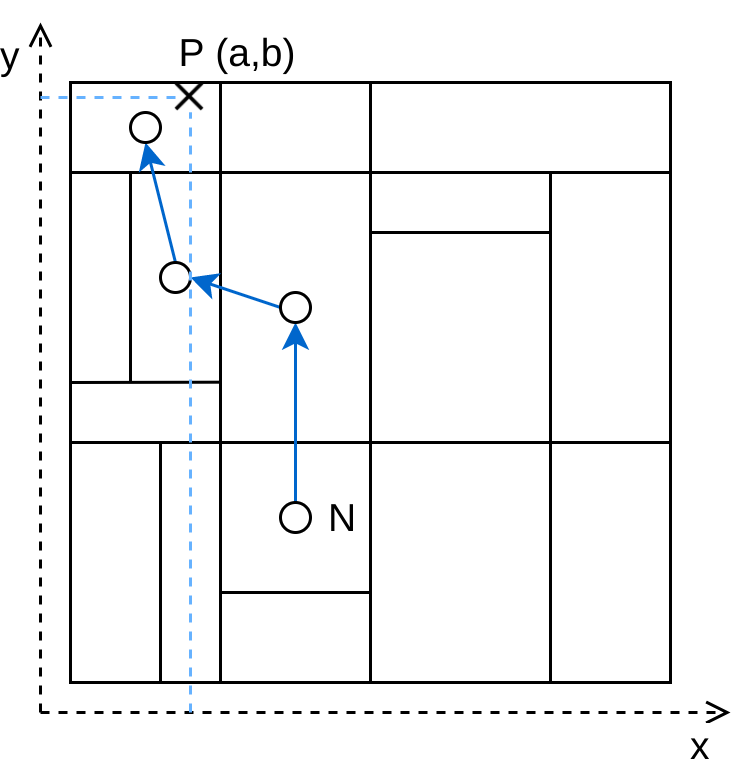
\includegraphics[max height=5cm,max width=0.95\textwidth]{img/can.png}
  \caption{Example of a 2 dimensional CAN routing command}
  \label{fig:can}
\end{figure}

Other popular examples in the DHT field are \textbf{Pastry} \cite{Rowstron2001} and
\textbf{Tapestry} \cite{Zhao2006} (that we kept out for the sake of simplicity, although
a lot of the mechanisms described above apply to these). DHTs present a
set of interesting benefits, such as good routing performance (usually
logarithmic in the number of nodes), the limited size of state kept at
each node (usually logarithmic routing tables), a better support for
exact match and other complex queries and also present stronger
guarantees on message delivery. If the hashing function is properly
selected it can also be ensured that the load is balanced properly
across the network. However, these networks lack the tolerance for heavy
network partitions and network churn that the usual unstructured network
can bare with.
\bigskip

\textbf{Hybrid overlays}: As with everything discussed so far, not every
solution lies at each end of the spectrum, and overlay structure is no
different. Recent research has been pushing more and more towards hybrid
solutions that take advantages of both sides. Such example is
\textbf{Vicinity} \cite{Voulgaris2013} which employs Cyclon
(discussed above) as a peer sampling service to help out in building an
ideal structure that links nodes based on their proximity (for some
notion of proximity, e.g.~latency, localisation, etc.). In the end, we
get a structured overlay, generated from an unstructured, gossip based,
overlay (hence the hybrid solution). More importantly, this overlay will
have properties that guarantee that it is an almost ideal structure for
a given proximity metric. The Vicinity system discusses that the usage
of probabilistic mechanisms helps out in keeping a healthy and reliable
structure.

\subsection{Subscription Management and Event
Dissemination}\label{subscription-management-and-event-dissemination}

Now that we have set the underlying structures that power up the
network, it is time to cover the specific requirements of a pub-sub
system. We have two different aspects to cover: subscription management
and event dissemination. By subscription management we refer to a set of
key factors that will determine the overall performance of the pub-sub
system, specifically in terms of matching events with subscribers, the
selected representation for subscriptions, registering new subscriptions
and deleting subscriptions. Event dissemination dictates how will the
events be propagated through the system, in a way that avoids burdening
specific nodes, but assures that all the subscription requirements are
met. It is natural that in some ways these two aspects are connected
(e.g.~the way we store our subscriptions will probably impose a set of
restrictions on how our events will be propagated) but it is still
possible to make a clear distinction between how they work and their
role in the overall system.

As discussed before, in order to match subscribers with publishers, some
kind of state must be kept (what we refer to as subscriptions). There are
plenty of ways of doing this and factors like network architecture and
subscription model come into play here. For a system with a centralised
architecture, this is not such a big challenge, since the central nodes
will be responsible for keeping and managing the state, matching events
with the correct subscribers and making sure the event propagation works
accordingly. However, in a distributed or a decentralised scenario, this
is not such a trivial problem to solve.

One interesting property of topic based systems in a decentralised and
distributed scenario is that their subscription management and event
dissemination can be easily implemented with an application level
multicast system if we cluster subscribers of some topic/group in a
single structure (e.g.~a multicast tree). For example, consider the
topic \emph{/foobar} issued by a particular node in a pub-sub system.
If, when new subscriptions are issued to this node, a tree like
structure is built that allows events related to this topic to flow
accordingly, disseminating a new event in \emph{/foobar} is just a
matter of sending the event to the root of the tree. From there,
dissemination can flow blindly through the multiple links. Subscriptions
are then represented as simple dissemination trees for each topic,
which, interestingly enough, ends up also representing how the actual
events will be propagated in each topic. The root node (or nodes) acts
as a \emph{rendezvous} which, as the name suggests, it is where events
are targeted at and new subscriptions issued to. The core idea is that,
by relying on such nodes, eventually, all the system state will be
synchronised (all the events will be propagated to the expected nodes
and no subscription is left unattended). This does not mean that other
nodes cannot cache state though, the idea of the \emph{rendezvous} is to
have a basic reassurance in subscription management and event
dissemination. Ideally this would be implemented in a distributed
fashion, keeping as much pressure out of the \emph{rendezvous} node as
possible. This is the approach followed by Scribe and Bayeux.

The usage of \emph{rendezvous} nodes and tree like structures to
represent subscriptions is not something particular to topic based
systems. There are examples of these techniques in content based systems
also, specifically Gryphon and Jedi. Hermes, on the other hand, is
an example of the same mechanisms with a type based subscription model.
A more detailed description of how this is done in Gryphon and Scribe
will be made further along since they have different approaches
motivated by their different options in network architecture and
subscription model.

For content based systems though, a common approach is to use
multidimensional spaces as a way to represent subscriptions. The idea is
to have each dimension refer to a specific attribute of the pub-sub
schema.

\begin{verbatim}
{
  exchange: String,
  company: String,
  order: String,
  number: Integer,
  price: Float,
}
\end{verbatim}

Considering the example above, we could map each of the given attributes
to a given dimension and end up with a 5 dimensional space that we could
use to route events accordingly. Meghdoot is an example of a content based
pub-sub system that follows an approach close to this one,
using a CAN DHT with $2n$ dimensions, where $n$ is the
number of attributes in the schema. We will cover Meghdoot further down,
but it is worth mentioning that there are other alternatives to using a
multidimensional space DHT to replicate this behaviour. Mercury
for example relies on the usage of several ring-based
DHTs to recreate this multidimensional space and support range queries,
using one DHT per attribute.

A different approach to managing subscriptions and disseminating events in
topic based systems is by having an overlay for each different topic.  The idea
is that by clustering nodes one can afford an easier event dissemination as
well as an easy way of matching events with subscribers, since it is just a
matter of propagating a given event inside its overlay. In order to keep
everything connected, a general overlay can be used, that will allow all the
nodes to have visibility on the whole set of topics. In this scenario,
subscriptions are simply represented as being part of a specific network of
peers, that could take any form or shape, or even be unstructured. For an
unstructured network, the propagation of events could be a simple flooding
algorithm, as it happens in Tera. Tera, a topic based pub-sub system, follows
an approach close to this one. It keeps two distinct gossip based overlays, one
responsible for keeping state on entrypoints for each topic (peers which are
subscribed to a given topic and that can act as dissemination points for it)
and another used to keep the subscribers of each topic. This clustering
approach, where subscribers of a given topic are kept in a topic specific
overlay, helps out in the dissemination step after an event has been published
and reached the cluster. Another example following this approach is Poldercast,
which uses a set of three different overlays to keep the pub-sub network
running. We will cover Poldercast more thoroughly later on.

\section{Relevant Pub-Sub
Systems}\label{relevant-pub-sub-systems}

We now describe in further detail the systems which most resemble the
work we are going to do.

\subsection{Gryphon}\label{gryphon}

Gryphon \cite{Strom1998} is a content based pub-sub system
built on top of a centralised broker hierarchy topology. Developed at
IBM, Gryphon uses an interesting approach to match events with
subscriptions \cite{Aguilera1999}. Gryphon relied on a distributed broker based
network to build a tree structure representing the
subscription schema. Considering a schema with multiple attributes -
$A1,\ldots{},An$ - each level on the subscription tree would represent a
specific attribute. So, for example, if we were to have an event with a
value $V1$ for the attribute $A1$, at the root node (which represents the
attribute $A1$) the link followed by the event would be the one that would
represent the value $V1$. The event would then be propagated through the
multiple branches of the tree until it arrives at the broker node that
represented all the specific values for that event. From there it would
then be propagated to all the subscribers registered with that broker
node. Figure \ref{fig:gryphon} illustrates this approach.

\begin{figure}[hb!]
  \centering
  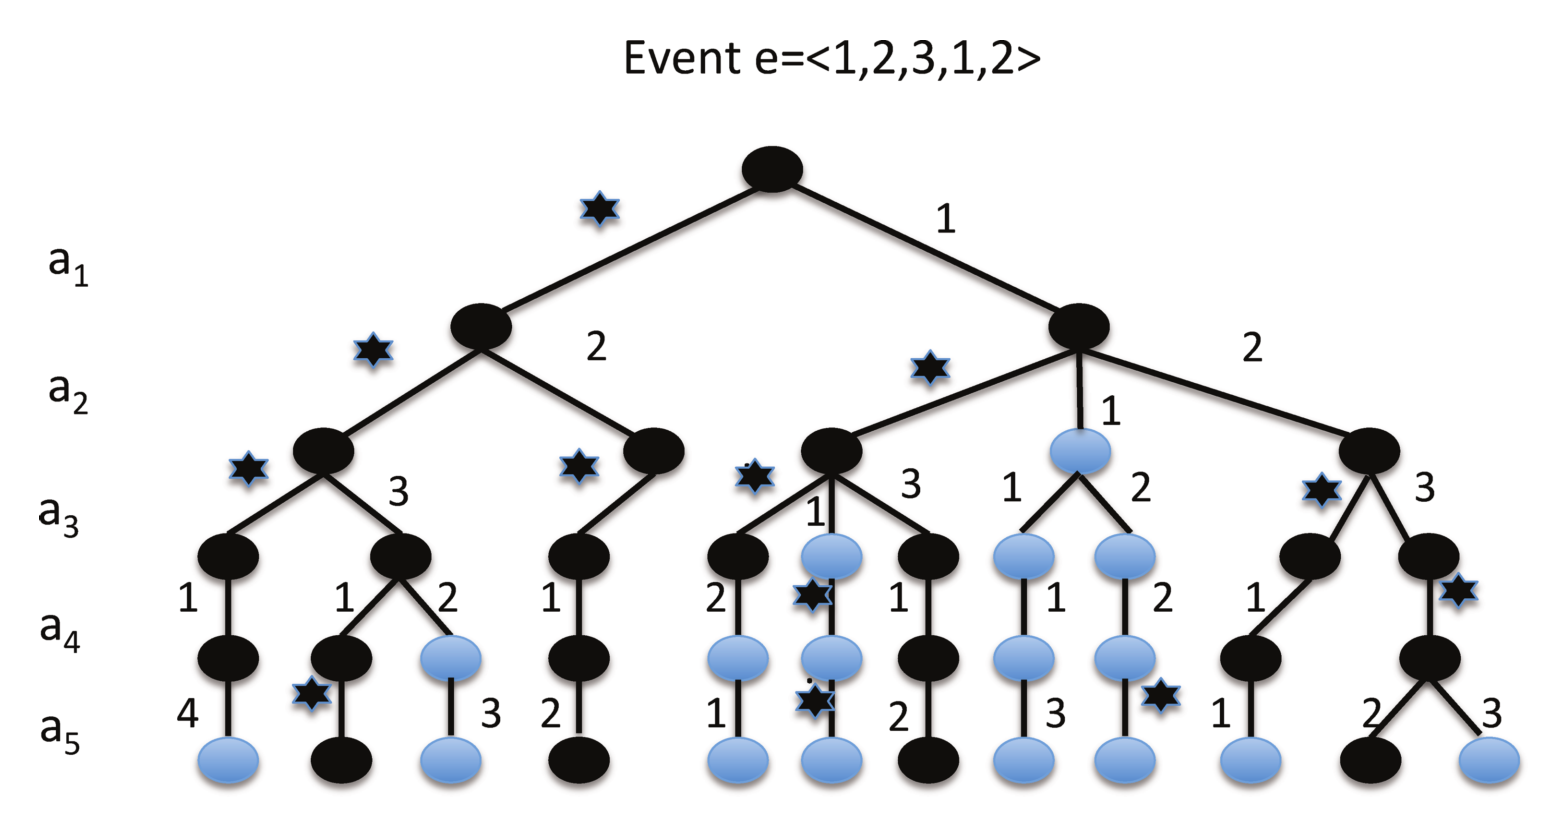
\includegraphics[width=0.95\textwidth]{img/gryphon.png}
  \caption{extracted from \cite{Kermarrec2013}. Each level of the broker tree represents an attribute.
  When the event $e = <1, 2, 3, 1, 2>$ is published,
  all dark circles (representing brokers) are visited.}
  \label{fig:gryphon}
\end{figure}

When a client issues a new subscription, the same approach will be
followed until the subscription arrives at the broker node that
represents it. If for some reason, the tree does not have an edge for a
specific value of an attribute, a new edge will be created. During both
of these approaches (subscription and event propagation), a subscription
or event that does not name an attribute at a given level will follow
the edge with label $*$ (do not care).

Gryphon has been successfully deployed over the Internet for real-time
sports score distribution at the Grand Slam Tennis events, Ryder Cup,
and for monitoring and statistics reporting at the Sydney Olympics~\footnote{https://www.research.ibm.com/distributedmessaging/gryphon.html}.

\subsection{Siena}\label{siena}

Siena \cite{Carzaniga2003} is a content based pub-sub system built
on top of a centralised broker mesh topology. Siena does not make any
assumptions on how the communication between servers and client-server
works, as this is not vital for the system to work. Instead, for server
to server communication, it provides a set of options ranging from P2P
communication to a more hierarchical structure, each with its respective
advantages and shortcomings.

Events in Siena are treated as a set of typed attributes with values.
Consequently, subscriptions (or \emph{event filters} as they are
referred to in Siena) select events by specifying a set of attributes
and constraints on its values. When issuing a new subscription, a client
sends its subscription to its broker node, which then forwards it
throughout the network. At each node, the subscription leaves some state
behind, identifying it and the neighbour which previously forwarded the
message. This is crucial, for these will be the dissemination paths that
events will follow when travelling through the network. Siena also
defines an interesting concept of \emph{subscription coverage}. A
subscription \emph{S} is covered by a subscription \emph{M} if, whenever
\emph{S} is matched by an event \emph{e}, then \emph{M} is matched by
\emph{e} as well. Although a simple concept, it saves a considerable
overhead during subscription dissemination and processing. A broker that
detects a link with a more general subscription will not need to forward
subscriptions that are covered by it.

Event dissemination will work based on the previously set state at each
broker node. In the end, events will technically follow the reverse paths
of the subscriptions. A detail worth noting is that Siena optimises for
\emph{downstream replication}, that is, events should be routed as one
copy as far as possible and should replicate only downstream.

Interestingly enough Siena also proposed another influential idea, which
is the idea of \emph{advertisements}. This concept could be viewed as a
reverse subscription. The concept is simple, a node advertises to the
network the type of content it is producing. In this paradigm,
advertisements are propagated throughout the network and when a
subscription is issued, it follows the paths previously set by the
advertisements, effectively \emph{activating} the path. Events are then
forwarded through these activated paths.

\subsection{Scribe}\label{scribe}

Scribe \cite{Castro2002} is a topic based pub-sub system built
on top of a fully decentralised network (P2P). In order to do this, it
relies on Pastry DHT as its overlay structure. This allows it to
leverage the robustness, self-organisation, locality and reliability
properties of Pastry. Pastry DHT is at all similar to the DHTs described
in the previous section (Chord and Kademlia), with a specific effort on
achieving good network locality and a routing mechanism close to that of
Kademlia.

Scribe subscriptions are represented by a multicast tree, with each
different tree representing a specific topic (or \emph{group} as it is
referred in Scribe). The root of this tree acts as the \emph{rendezvous}
node for the group. Each group has a \emph{groupId} assigned to it, as
such, the \emph{rendezvous} node will be the one with the closest ID in
the network. This multicast tree is built by joining the multiple Pastry
routes from each group member to the \emph{rendezvous}. This dynamic
process happens whenever a new node decides to join a group. In order to
do that, it asks Pastry to route a \emph{JOIN} message with the
\emph{groupId} as the key. At each node along the path, the Scribe
forward method is invoked to check this node is already part of this
group (also called a \emph{forwarder}). If it is, it accepts the
\emph{JOIN} request and sets the node as its child, else this node will
become a \emph{forwarder} for the group, sets the requesting node as its
child and it sends a \emph{JOIN} request to this group. Note that any
node can be a \emph{forwarder} for any group, it does not need to be an active
part of it (i.e.~subscriber or publisher).

Disseminating an event in a group is a matter of disseminating it
through its respective multicast tree. Fault tolerance mechanisms can be
implemented on top of this system but, out of the box, Scribe provides
only best effort delivery. As for the \emph{rendezvous} nodes, their
state can be replicated across the k closest nodes in the leaf set of
the root node. Whenever a failure is detected by one of the children, it will
issue a \emph{JOIN} message which, thanks to Pastry's properties will be
routed to a new root node which has access to the previous state of the
\emph{rendezvous}.

\subsection{Meghdoot}\label{meghdoot}

Meghdoot \cite{Gupta2004} is a content based pub-sub system.
It is built on top of a P2P network, specifically CAN DHT (already
covered in the previous section). Meghdoot leverages the
multidimensional space provided by the CAN DHT in order to create an
expressive content based system.

In Meghdoot, subscriptions are defined over a schema of \emph{n}
attributes. Each attribute has a \emph{name}, \emph{type}, and
\emph{domain}, and can be described by a tuple
\emph{\{Name:\ Type,\ Min,\ Max\}}. \emph{Min} and \emph{Max} describe
the range of domain values taken by the given attribute. All the peers
in the system will use this same model. A subscription will then be a
set of predicates over the previously defined attributes. In order to
map this to the CAN DHT, Meghdoot defines the $n$ attributes schema
as a $2n$ dimensional space in the DHT. Subscriptions will be a
point in this multidimensional space, where the range query it defines
will be represented as two separate dimensions per attribute in the DHT
(hence the $2n$ space). Each subscription is routed through the CAN
DHT until it reaches the peer responsible for managing the zone it is
part of.

Event dissemination in Meghdoot will be a matter of routing each event
through the CAN DHT. The events too will be defined by points in the
multidimensional space. The point will be represented by the value of
that same attribute in each of dimensions used to map it. For example,
for a 2 dimensional space $(x,y)$ (only one attribute), an event
with a value $z$ would be mapped to a point $x=y=z$. Once the
event arrives at the node responsible for managing that specific zone in
the DHT, it will be up to it to route the event to all of its neighbours
that are part of the region affected by it. An interesting property of
the $2n$ dimensional space is that half of it is left unexplored by
the default subscription algorithm. This allows that space to be used to persist
replicas of the subscriptions on the other half, making Meghdoot a
system with fault tolerance by default.

\subsection{Poldercast}\label{poldercast}

Poldercast \cite{Setty2012} is a recent pub-sub system with
a strong focus on scalability, robustness, efficiency and fault
tolerance. It follows a topic based model and follows a fully
decentralised architecture. The key detail about this system is that it
tries to blend deterministic propagation over a structured overlay, with
probabilistic dissemination through gossip based unstructured overlays.
In order to do this, Poldercast uses 3 different overlays. Two of them,
Cyclon and Vicinity, we covered in the previous section and the third
one closely resembles Chord in many ways.

Poldercast subscriptions are represented as a structured ring overlay.
Each topic has its own overlay in fact, with all subscribers (and only
them) of the corresponding topic connected to it. This overlay is
maintained by a module referred to as the \emph{Rings Module} and its
overall mechanisms closely resemble Chord's ones. In order for each node
to have visibility across the whole pub-sub network, Vicinity, with the
help of Cyclon, will be responsible for keeping an updated set of peers
participating in each of the available topics in the network.
Subscribing to a topic will then be a matter of consulting this set of
peers and joining the specific overlay for the topic.

Propagating events will be a matter of forwarding the event through the
specific topic overlay. It is important to notice that Poldercast
assumes only peers subscribed to a topic can publish to that same topic.
The way this propagation works is through the ring overlay that, despite
being similar to Chord, it has some important differences. It does not
use a finger table at each node to speed up propagation. Instead, with
the help of Vicinity, each node keeps a random set of peers for the
topics it is part of. With them, whenever a node receives a message from
a specific topic, it will propagate the event through a set of these
peers. This propagation will be based on a system wide fanout parameter.
It will also forward the event to its successor or predecessor
(depending on where the event originated from), or will simply ignore if it
is not the first time it has received it. These mechanisms, depending on
the fanout parameter, guarantee average dissemination paths for each
topic to be asymptotically logarithmic.

Through the multiple mechanisms described above, Poldercast attempts to
provide a set of guarantees. To start with, only nodes subscribed to a
topic will receive events published to that topic. In other words, no
relay nodes are used. It also focuses on handling churn through the use
of a mixture of gossip mechanisms, ensuring a highly resilient network.
Finally, it seeks to reduce message duplication factor (i.e. nodes receiving
the same message more than once).

\subsection{Systems Analysis}\label{systems-overview}

Let us now analyse all the relevant pub-sub systems we used as a basis for our
work. Table \ref{table:relevant-systems} will serve as a useful comparison
mechanism for this.  A couple of notes on the terminology used. We refer to
\emph{delivery guarantees} as the ability to deliver a message under normal
working conditions and \emph{fault tolerance} as the ability to keep such
guarantees under churn. This, of course, depends on the persistence of
subscriptions and mechanisms to replicate these. The rest of the criteria were
addressed in the previous sections.

\begin{sidewaystable}
  \center
    \begin{tabular}{|P{3cm}|P{2cm}P{2cm}P{2cm}P{2.5cm}P{2cm}P{2cm}P{2cm}P{2cm}|}\hline
    Systems / Properties & Subscription Model & Architecture & Overlay Structure & Subscription Management & Event dissemination & Relay Free Routing & Delivery Guarantees & Fault Tolerance \\\hline
    Gryphon & Content based & Centralised broker hierarchy & N/A & Each broker responsible for a subscription scheme & Tree hierarchy & N/A & Yes & Best effort \\\hline
    Siena & Content based & Centralised broker mesh & N/A & Keep state at each node & Flood with cached state & N/A & Yes & Best effort \\\hline
    Jedi & Content based & Centralised broker hierarchy & N/A & Keep state at each node & Tree hierarchy & N/A & Yes & Best effort \\\hline
    Bayeux & Topic based & Decentralised & Tapestry DHT & Rendezvous node & Multicast tree & No & Yes & Best effort, no subscription persistence \\\hline
    Scribe & Topic based & Decentralised & Pastry DHT & Rendezvous node & Multicast tree & No & Yes & Best effort, no subscription persistence \\\hline
    Medhdoot & Content based & Decentralised & CAN DHT & Points in CAN DHT & CAN routing  & No & Yes & replicated subscriptions \\\hline
    Hermes & Type based & Decentralised & Pastry DHT & Rendezvous node & Multicast tree & No & Yes & Best effort \\\hline
    Tera & Topic based & Decentralised & Gossip based overlay & Unstructured overlay per topic & Random walks and flooding & No & no & Best effort \\\hline
    Mercury & Content based & Decentralised & Ring based DHTs & Overlay per attribute in schema & Route through ring overlays & No & Yes & Best effort \\\hline
    Sub-2-Sub & Content based & Decentralised & Ring based DHT and gossip based overlay & Clustering of similar subscriptions & Gossip and ring overlay routing & No & No & Best effort \\\hline
    Poldercast & Topic based & Decentralised & Ring based DHT/ Vicinity / Cyclon & Ring overlay per topic & Ring overlay routing & Yes & Yes (every publisher is a subscriber) & High resilience to churn, no subscription persistence \\\hline
    \end{tabular}
  \caption{Comparison table for the relevant system}
  \label{table:relevant-systems}
\end{sidewaystable}
\section{Web Technologies}\label{web-technologies}

When building any kind of network focused system nowadays, there is no question
that one should take advantage of the full potential that the web has to offer.
Browsers evolved a lot over the past years and allow for a vast world of
possibilities in terms of applications that can be built on top of it. P2P
applications are no exception here. In the next sections, we will cover a set
of technologies that allow for a modern distributed application to run, not
only on the desktops and servers we are used, but also in browsers running in
multiple platforms.

It is indisputable that one cannot think of modern web development
without speaking of \textbf{Javascript}~\footnote{https://www.ecma-international.org/publications/standards/Ecma-262.htm}.
Javascript is a lightweight, interpreted, programming language, known as
the scripting language for the web. Initially created with the purpose
of allowing the creation of simple interactions and animations in web
pages it is now one of the main programming languages for the web
~\footnote{https://insights.stackoverflow.com/survey/2017}. It is used, not
only for client side programming but also to power server side
applications. Since Javascript has different runtimes, it became
necessary to create a standardised base from which the multiple browser
vendors and runtime maintainers could work from. Hence ECMAScript, the standard
for the Javascript implementation.

As it was previously said, nowadays, Javascript is not restricted to
browsers only. \textbf{NodeJS}~\footnote{https://nodejs.org} was the first
successful implementation of a Javascript runtime for the server, built
on top of Chrome's V8 JavaScript engine~\footnote{https://developers.google.com/v8/}. This
allowed developers to write and run Javascript programs in multiple
architectures and operating systems, with access to a set of common
native libraries that allow to interact with relevant parts of the
system~\footnote{https://nodejs.org/api/} such as network, filesystem and
others. A key aspect in NodeJS was the way it chose to deal with the
lack of support from Javascript for multithreading: the use of an event
loop that powers an event-driven architecture capable of asynchronous
I/O.

Yet another key element in the NodeJS and Javascript ecosystem is
\textbf{NPM}~\footnote{https://www.npmjs.com/}, its package manager. NPM was one
of the main drivers of a philosophy that is deeply ingrained in the JS
ecosystem which focuses on building small reusable packages that
everyone can use and build on top of. This is heavily inspired by the
UNIX philosophy summarised by Doug McIlroy~\footnote{https://archive.org/details/bstj57-6-1899} - "Write
programs that do one thing and do it well. Write programs that work
together". This approach ended up being a major differentiator on how
modern web applications are developed. Currently, NPM is one of the
largest package registries in the world~\footnote{http://blog.npmjs.org/post/143451680695/how-many-npm-users-are-there}.
This mindset though is really important, for it allows applications to
be built on top of previously published packages, making modularity and
code reusability core values of the ecosystem. Even more interesting is
the sudden possibility offered by having the same programming language
supporting different environments (browsers, servers, desktops, etc.),
all of this powered by a common way of publishing and sharing code.

When focusing specifically on P2P apps, the past years have brought
together a set of new network protocols that empower communication
between browsers in a real-time fashion and also provide alternatives to
TCP~\footnote{https://tools.ietf.org/html/rfc793}. \textbf{WebSockets}~\footnote{https://tools.ietf.org/html/rfc6455}
aimed at providing a real-time, full-duplex communication
between clients and servers over TCP, but it was \textbf{WebRTC}~\footnote{https://www.w3.org/TR/webrtc/}
that paved the way for new P2P applications that could
run in the browser. WebRTC focuses on powering real-time communications,
like audio/video stream or just arbitrary data, between browsers,
without the need of an intermediary. This, of course, is a real
breakthrough in the P2P field as it allows browsers to receive incoming
connections. On other hand, alternatives to the TCP transport, such as
\textbf{uTP}~\footnote{http://www.bittorrent.org/beps/bep\_0029.html} and
\textbf{QUIC}~\footnote{https://datatracker.ietf.org/wg/quic/about/}
, came through, seeking to bring reliability and order delivery
without the poor latency and congestion control issues of TCP. This
provided new suitable alternatives to communication between peers on top
of UDP, a transport that has been vital in P2P applications that need an
affordable way to perform NAT~\footnote{https://tools.ietf.org/html/rfc2663} traversal.

In the application realm, there have been quite a few in the past years
that seek to leverage all these new technologies and breakthroughs. One
of the examples most worth mentioning is the \textbf{InterPlanetary File
System} (IPFS)~\footnote{https://ipfs.io}, a P2P hypermedia protocol designed
to create a persistent, content-addressable network on top of the
distributed web.

At the core of IPFS is what they refer to as the \textbf{Merkle
DAG}~\footnote{https://github.com/ipld/specs/blob/95df205ca5fdb961ec2c2265a169989fef595db1/FOUNDATIONS.md}.
The Merkle DAG is a graph structure used to store and represent data, where
each node can be linked to based on the hash of its content. Figure
\ref{fig:merkle-node} provides an example of this. 

\begin{figure}[hb!]
  \centering
  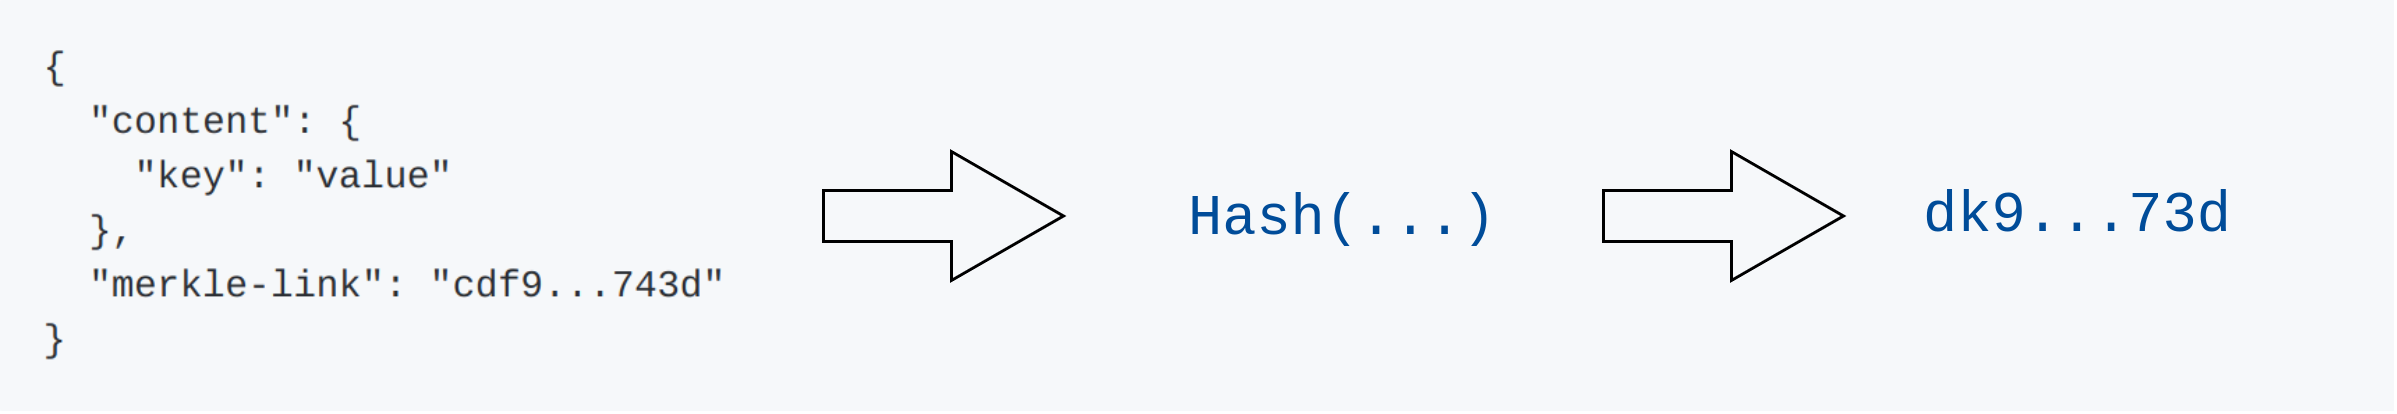
\includegraphics[max height=5cm,max width=0.95\textwidth]{img/merkle-node.png}
  \caption{JSON representation of a Merkle node with a Merkle link}
  \label{fig:merkle-node}
\end{figure}

Each node can have links (Merkle links) to other nodes, creating a persistent,
chain like, structure that is immutable as documented in figure
\ref{fig:merkle-dag}

\begin{figure}[hb!]
  \centering
  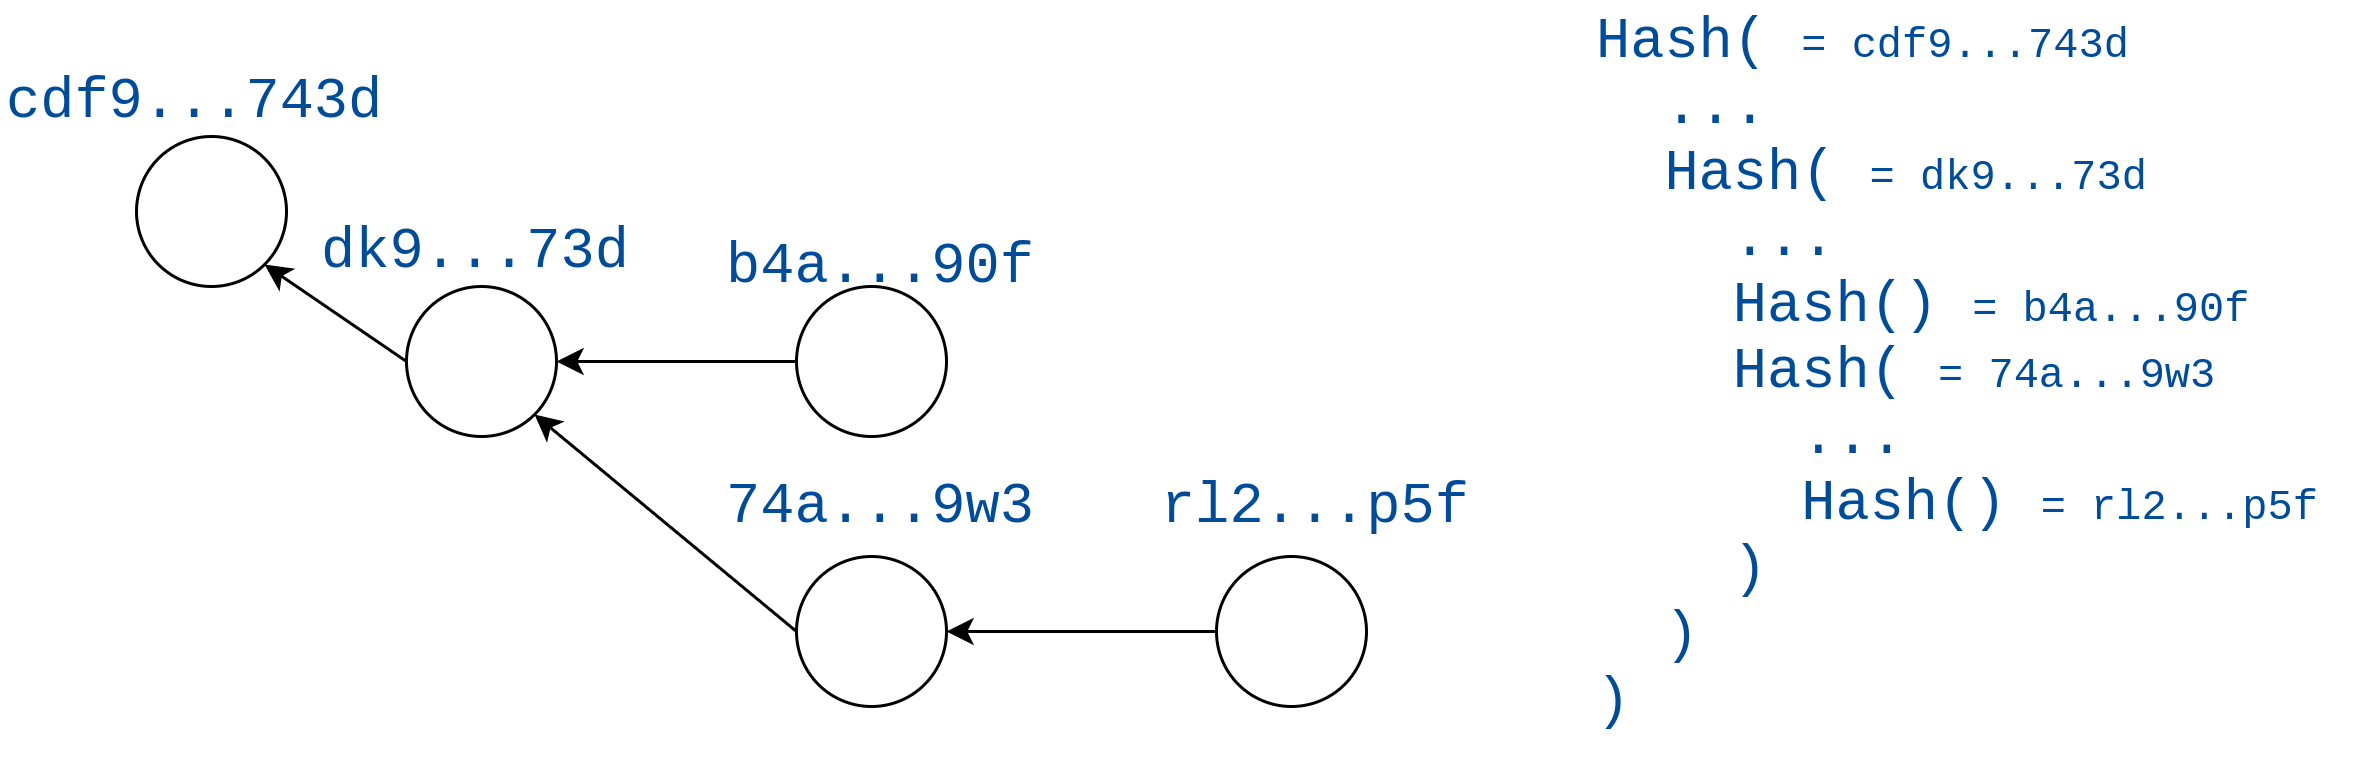
\includegraphics[max height=5cm,max width=0.95\textwidth]{img/merkle-dag.png}
  \caption{Graph visualisation of a Merkle DAG and its respective hash function dependencies}
  \label{fig:merkle-dag}
\end{figure}

IPFS has an interface around this structure referred to as
\textbf{InterPlanetary Linked Data} (IPLD)
which focuses on bringing together all the hash-linked data structures
(e.g.~git) under a unified JSON-based model. In order
to interact with IPLD, IPFS exposes an API that allows us to insert and
request random blobs of data, files, JSON objects and other complex
structures. Having implementations in both Go and
Javascript, IPFS leverages the modularity mantra in a fascinating way,
focusing on creating common interfaces that allow for different pieces
of the architecture to be changed and selected according to one's needs.
All of this without impacting the overall application and its top level API.
These came from the observation that the web we have today is a set of
different heterogeneous clients, that have different needs and resources. As
such, not everyone can rely on the same set of transports, storage management
and discovery mechanisms. These small modules that constitute IPFS have
recently been brought together under the same umbrella, as
\textbf{libp2p}~\footnote{https://libp2p.io}, a set of packages that seek to
solve common challenges in P2P applications. 

\begin{figure}[hb!]
  \centering
  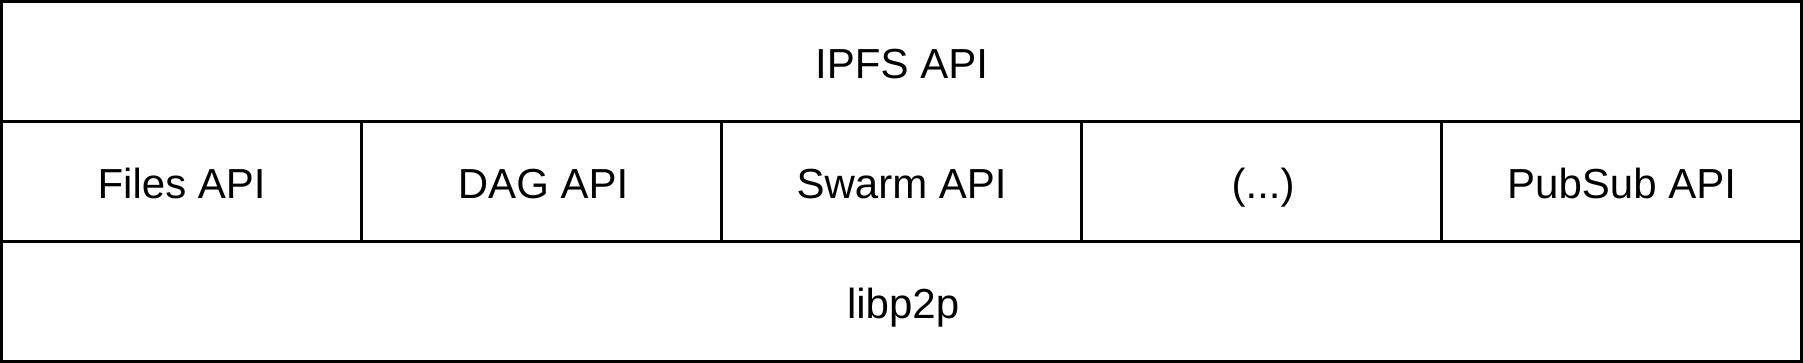
\includegraphics[width=0.95\textwidth]{img/ipfs-stack.png}
  \caption{An illustration on the IPFS architecture}
  \label{fig:ipfs-stack}
\end{figure}

Interestingly enough, a recent addition to libp2p, and consequently IPFS, was a
pub-sub module, with a naive implementation using a simple network flooding
technique. Even though libp2p was created with the initial purpose of serving
as the foundation of IPFS it is now possible to use libp2p as a standalone
module for peer to peer apps, with the possibility to hand pick the
functionalities we intend to use.

\begin{figure}[hb!]
  \centering
  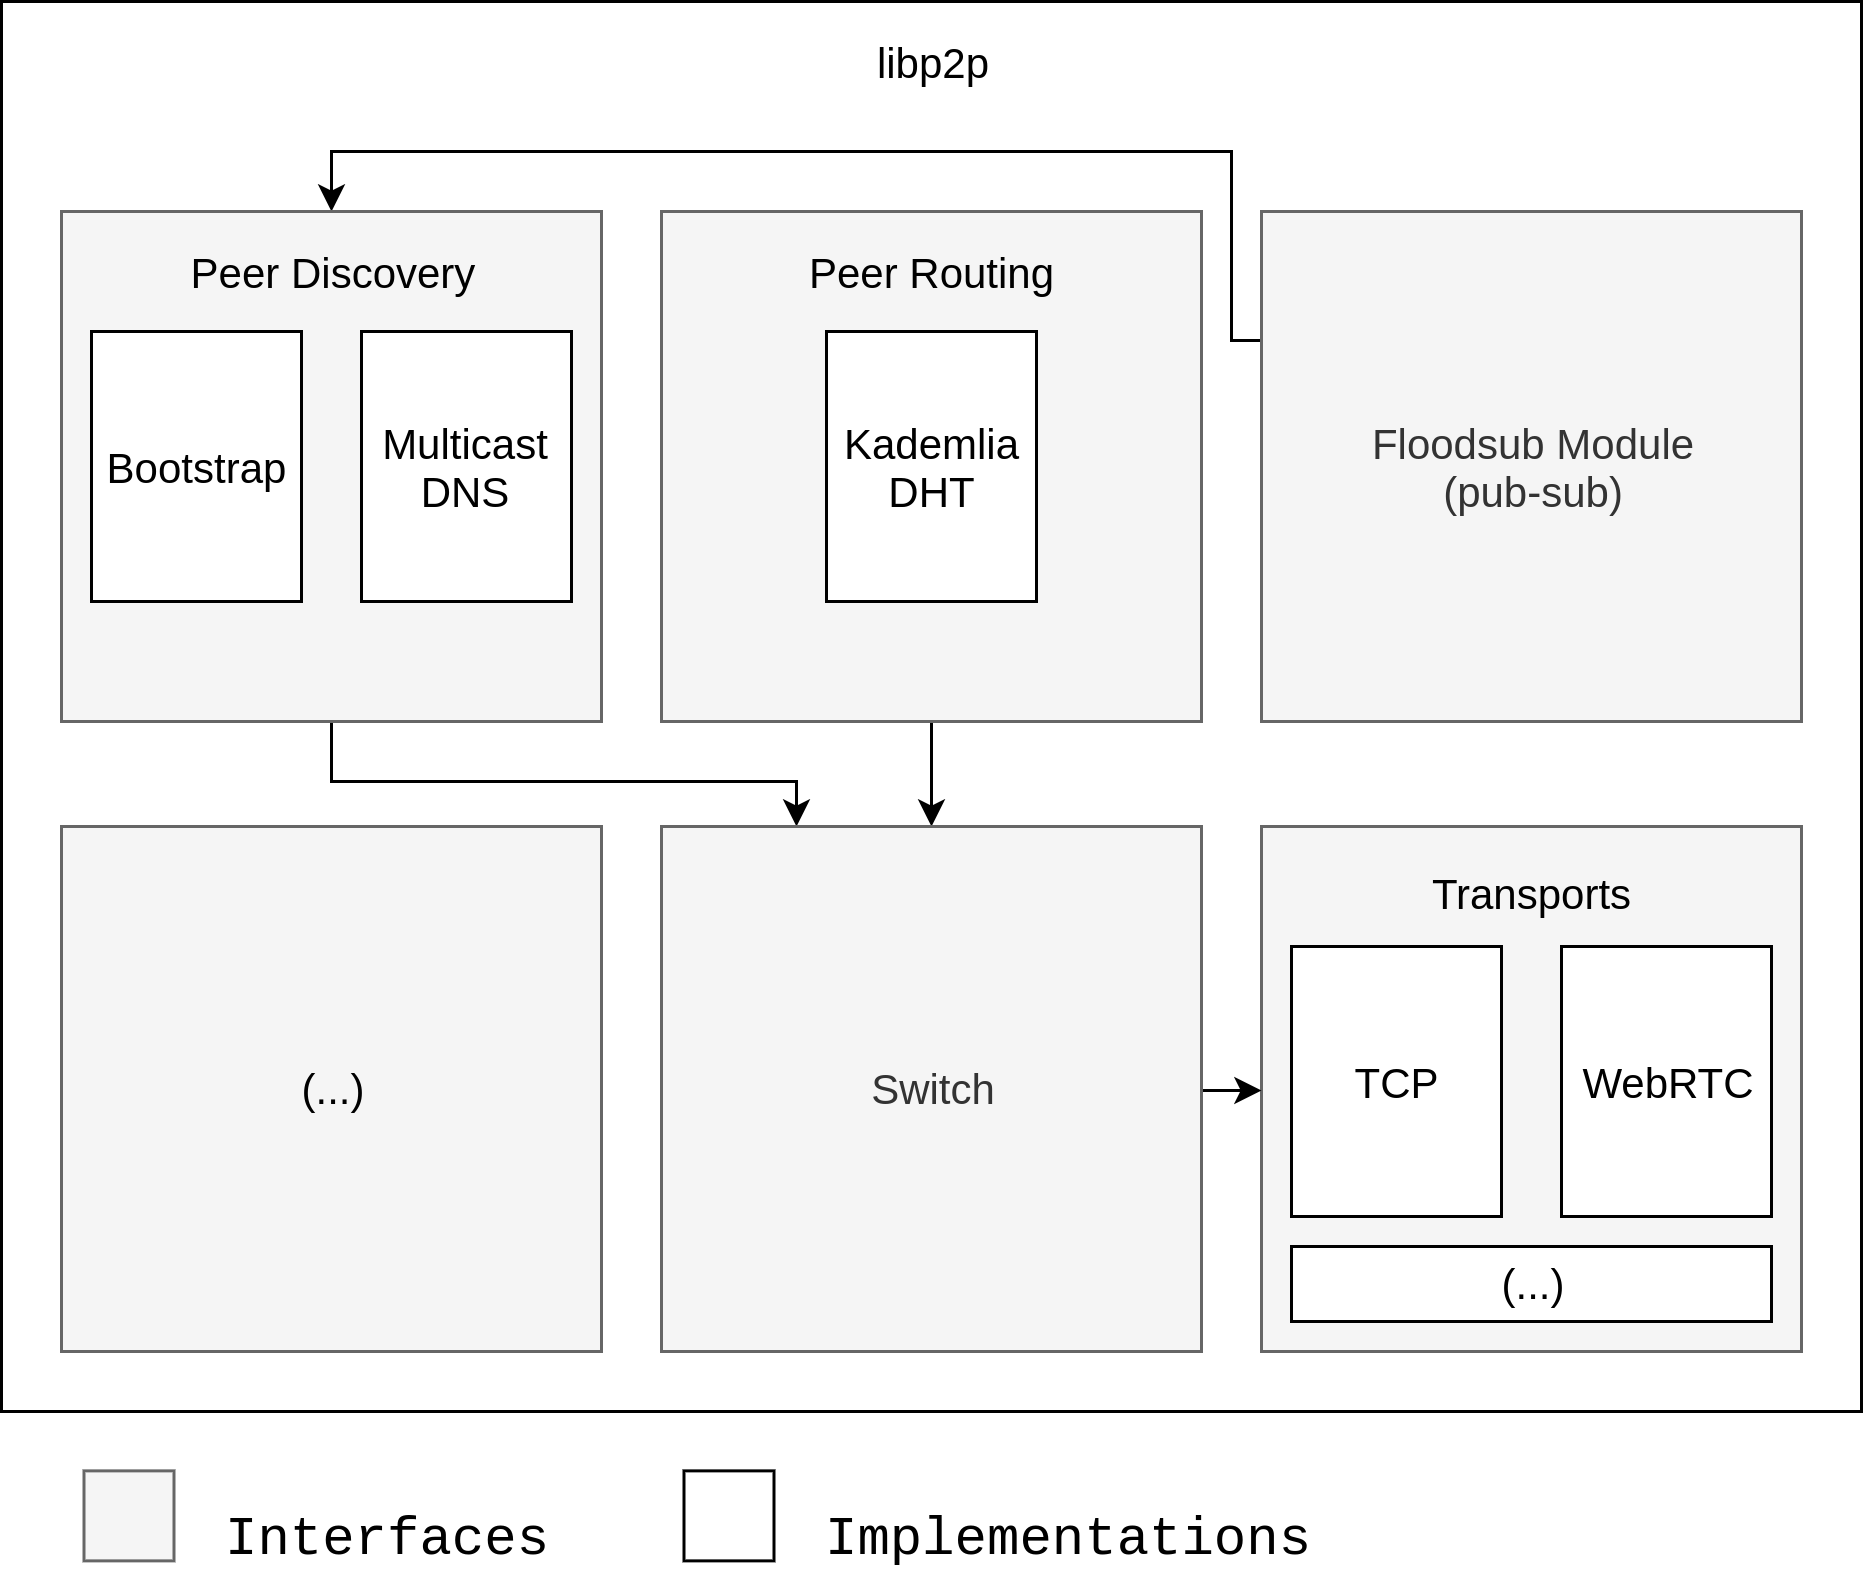
\includegraphics[width=0.95\textwidth]{img/libp2p-arch.png}
  \caption{An illustration on the libp2p architecture}
  \label{fig:ipfs-arch}
\end{figure}

\section{Summary}\label{summary}

TODO

